\documentclass[tikz,border=8pt]{standalone}
% Shared look for every TikZ diagram. Load with \input{../../tools/tikz-style.tex}
\usepackage[T1]{fontenc}
\usepackage{lmodern}
\renewcommand{\sfdefault}{lmr}  % diagrams use the same serif as the text
\usetikzlibrary{arrows.meta, positioning, shapes.geometric, calc, fit, backgrounds}
\definecolor{cblue}{HTML}{4C78A8}
\definecolor{corange}{HTML}{F58518}
\definecolor{cgreen}{HTML}{54A24B}
\definecolor{cred}{HTML}{E45756}
\definecolor{cpurple}{HTML}{B279A2}
\definecolor{cgrey}{HTML}{6B6B6B}
\tikzset{
  every picture/.style={font=\sffamily, line width=1.2pt},
  box/.style={draw=#1, fill=#1!12, rounded corners=4pt, align=center, inner sep=7pt, minimum height=1.1cm},
  box/.default=cgrey,
  arrow/.style={-{Stealth[length=3mm]}, draw=cgrey, line width=1.4pt},
  title/.style={font=\sffamily\bfseries\Large},
  note/.style={font=\sffamily\small, text=cgrey, align=center},
}
\AtBeginDocument{\hyphenpenalty=10000 \exhyphenpenalty=10000}

% Velocity v = 0.5 m/s at heading 30 degrees split into x part v cos(theta) = 0.433 and y part v sin(theta) = 0.25.
\begin{document}
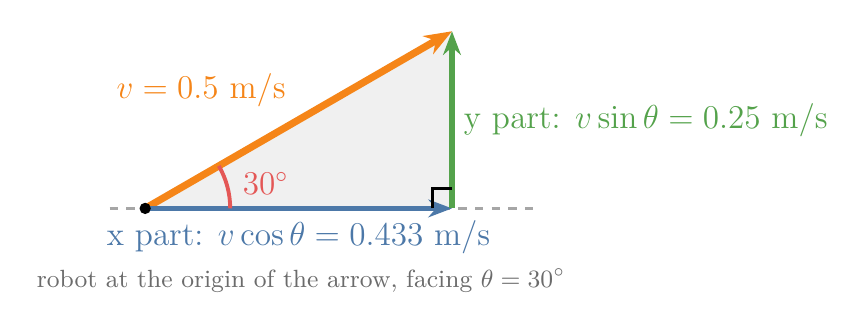
\begin{tikzpicture}[scale=9, every node/.append style={font=\large}]
  \coordinate (O) at (0,0); \coordinate (P) at (0.433,0.25); \coordinate (X) at (0.433,0);
  \draw[cgrey!60, line width=0.8pt, dashed] (-0.05,0) -- (0.55,0);
  \fill[cgrey!10] (O) -- (X) -- (P) -- cycle;
  \draw[-{Stealth[length=3.5mm]}, corange, line width=2.6pt] (O) -- (P) node[midway, above left] {$v = 0.5$ m/s};
  \draw[-{Stealth[length=3mm]}, cblue, line width=2pt] (O) -- (X) node[midway, below] {x part: $v\cos\theta = 0.433$ m/s};
  \draw[-{Stealth[length=3mm]}, cgreen, line width=2pt] (X) -- (P) node[midway, right] {y part: $v\sin\theta = 0.25$ m/s};
  \draw (0.405,0) -- (0.405,0.028) -- (0.433,0.028);
  \draw[cred, line width=1.4pt] (0.12,0) arc (0:30:0.12);
  \node[cred] at (0.17,0.035) {$30^\circ$};
  \fill[black] (O) circle (0.008);
  \node[note, below] at (0.22,-0.07) {robot at the origin of the arrow, facing $\theta = 30^\circ$};
\end{tikzpicture}
\end{document}
